\documentclass[10pt,journal,compsoc]{IEEEtran}
\usepackage[UKenglish]{babel}
\usepackage[utf8]{inputenc}

\usepackage{graphicx}
\usepackage{mathtools}
\usepackage{amsmath}
\usepackage{url}
\usepackage{listings}
\usepackage{float}
\usepackage{fancyvrb}
\usepackage{framed}
\usepackage{attrib}

\hyphenation{op-tical net-works semi-conduc-tor}

% Styling commands
\newcommand{\tbf}[1]{\textbf{#1}}
\newcommand{\tit}[1]{\textit{#1}}
\newcommand{\ttt}[1]{\texttt{#1}}

% Document-specific commands
\newcommand{\ws}{WebSocket}
\newcommand{\term}[1]{\tit{#1}}


\begin{document}

\author{\IEEEauthorblockN{Thibault Gérondal, Michaël Heraly}}

\title{Survey: \ws }

\date{Tuesday, 27 Oct 2015}


\maketitle
\IEEEpeerreviewmaketitle

\markboth{Université catholique de Louvain, October 2015}{}

%\IEEEdisplaynontitleabstractindextext

\begin{abstract}
The most common way to get information and to communicate through the internet is via the Hypertext Transfer Protocol (HTTP).
Over time, the shared media sent through this communication system has evolved, from text to images and videos.
Interactions between clients and servers have evolved as well.
We went from passive customers who receive information to active clients wanting to communicate in real-time.
The original HTTP was never designed to achieve those needs.
The market found some tricks to bypass these limitations.
However, the HTML5 initiative introduced a real solution to this problem : \ws{}.
This solution brings sockets to the web, so that full-duplex communications can be established between clients and servers.
% This paper is only bullshit, but let's try to sell it.

In this survey paper, we describe the older techniques that were used to achieve a full-duplex communication before describing the \ws{} protocol itself.
Then, we explore some experiments that show how \ws{} is more efficient than these older methods.
Finally, we discuss the security issues of \ws{}.
\end{abstract}


\section{Introduction}

The Hypertext Transfer Protocol (HTTP) is a stateless request-response protocol in the server-client computing model.
The client submits an HTTP request message and the server provides a response (HTML files, images, etc.).
With the growing popularity of the web, the number of web applications has risen significantly, and the need of interactivity between the client and the server has also increased. % has also increased, comme c'est la la suite du "has risen"
In the original HTTP specifications, interactivity was only possible by loading an entire page in order to upload information to the server or to receive new information from it. %to download ? et pas to recieve, comme tu dis to upload avant et pas to send
New features of web browsers have arisen in order to successfully add interactivity without (re)loading pages \cite{RealTimeMonitoringUsingAJAXAndWebSockets}.
Among these, two Javascript APIs were implemented successively in web \mbox{browsers :} XML\-Http\-Request and \ws. % two APIs on met le pluriel aux abbrevs


\section{XMLHttpRequest}
\label{XHR}
% Note: real-time interactivity?
One of the first and most used solutions to add real-time interactivity is the XMLHttpRequest (XHR) Object, which is a Javascript API that permits the browser to send an HTTP request to query a resource from a distant server. % that permits => that allows, from a resource? c'est normal ça :p c'est d'un élément d'une page?  (connais pas les termes du domaine, c'est possible)
Despite the name of this API, the fetched resource does not have to be an XML file. %the resource is being fetched here and it sends a request above?
In fact, JSON (JavaScript Object Notation) is generally used as it is easier to parse in JavaScript \cite{collinalatency}.
This technique is great to send data to the server but not for receiving new data.
If the client wants to keep the information up-to-date from the server, it will have to poll the server periodically.
This behavior generates a lot of overhead as each request and response will have a full HTTP header and a lot of those requests might return no new data. This technique thus proves to be quite ineffective. % overhead work/tasks/something? (ou rien si c'est habituel)

\subsection{The long polling version}

The XHR long polling exploits a loophole inside the \mbox{HTTP/1.1} specifications.
After receiving an HTTP request, a web server is not required to respond immediately, it can defer the reply for a few instants \cite{collinalatency}.
With this technique, the client does not have to poll the server periodically as the web server holds the HTTP request open until it has new data to send to the client, or until a timeout occurs.
This reduces the amount of useless data transfers and improves the update delay.

\begin{figure}[!ht]
  \centering
  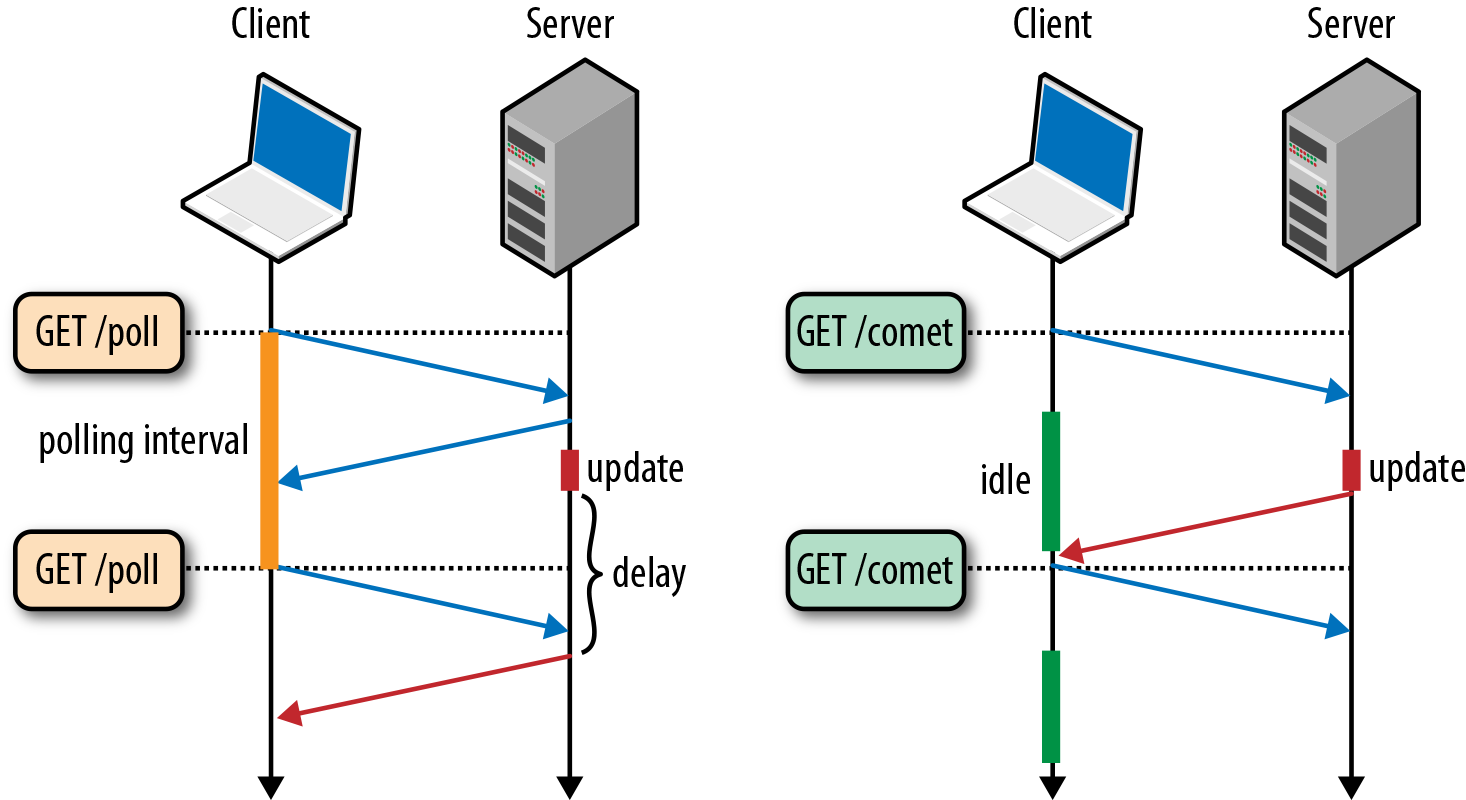
\includegraphics[width=\linewidth]{poll_vs_lpoll}
  \caption{periodic polling (left) versus long polling (right) (from \cite{HighPerfBrowserNetworking:polling})}
  \label{poll_vs_lpoll}
\end{figure}

In Fig.~\ref{poll_vs_lpoll}, on the left, the client periodically polls the server to retrieve updates. This is shown on the figure as the ``polling interval''. When an update occurs on the server side, the client has to wait for the next polling to become aware of it. On the right, with long polling, the server keeps the connection open until the update occurs. The periodic polling introduces a delay that long polling can avoid. Also, the first poll of the periodic polling is superfluous as it generates data on the network without any real new input. % pq polling au lieu de poll(s) parfois? the next poll, the first poll, ...

\section{\ws{} protocol}
\label{sec:ws}
The \ws{} protocol was standardized by the IETF as RFC 6455 in 2011 \cite{rfc6455}.
This protocol was designed to bring bidirectional, message-oriented streaming of texts and binary data between web browsers and web servers.

As it was designed for the Web, this protocol copes with existing HTTP infrastructures, which means working over HTTP ports 80 and 443.
As the \ws{} protocol is backward compatible with the existing Web infrastructure, it inherits all its benefits. % virer le from, it inherits benefits from it.
First of all, web browsers support the technology natively, including an origin-based security model. % Expliquer dans une section sécurité ?
The Web infrastructure provides URL-based endpoints, which allows to run multiple services on a single TCP port.
%It also removes the length limits imposed by plain TCP protocol.
Finally, it enables the traversal of proxies and firewalls.

The \ws{} protocol remains a fully functional protocol that can be used outside the browser.

\subsection{The \ws{} header}
\label{sec:ws-header}
The \ws{} frame structure is shown in Figure \ref{fig:websocket_frame}.

\begin{figure}
    \centering
    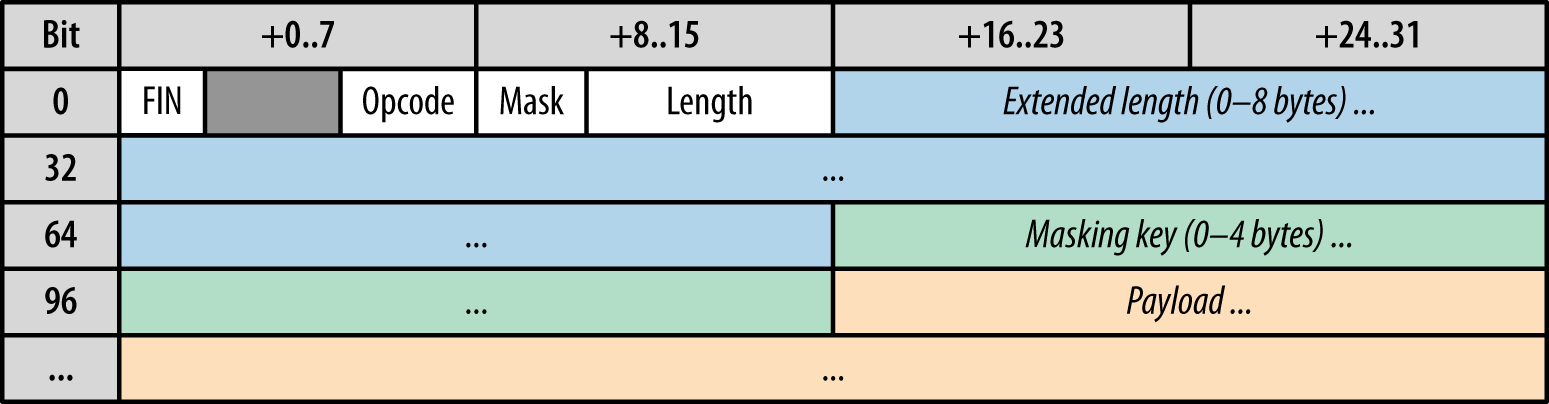
\includegraphics[width=\linewidth]{websocket_frame.png}
    \caption{\ws{} frame structure (from \cite{HighPerfBrowserNetworking:websocket})}
    \label{fig:websocket_frame}
\end{figure}

The \ws{} frame structure is composed of different parts \cite{HighPerfBrowserNetworking:websocket} \cite{performanceEvaluationOfWebsocketProtocol} :
\begin{LaTeXdescription}    % 'description' environment doesn't display well for IEEEtran
    \item[FIN] indicates whether the frame is the final fragment of a message. % THE final fragment, there is only one per message I assume?
    \item[Opcode] indicates the type of the payload data: binary, textual, or protocol-level signaling (e.g. \ttt{close}, \ttt{ping}, \ttt{pong}).
    \item[Mask] indicates whether the payload data is obfuscated (only for messages sent from the client to the server).
    \item[Length] indicates the payload length. If this value lies between 0 and 125, this is the actual length.
                    If it is set to 126, the next 2 bytes represent a 16-bit unsigned integer indicating the frame length.
                    If it is set to 127, the next 8 bytes represent a 64-bit unsigned integer indicating the frame length.
    \item[Masking key] is used to disable unwanted payload processed by network intermediaries, like HTTP proxies \cite{performanceEvaluationOfWebsocketProtocol}.
                    This part is omitted in server-originated frames, as the masking is not necessary. See section~\ref{sec:key} for more information.
    \item[Payload] corresponds to the application data, or custom data if the client and server use a protocol extension.
\end{LaTeXdescription}


%\section{\ws{} Javascript API}
%The \ws{} Javascript API is being standardized by the World Wide Web Consortium (W3C).


\subsection{The \ws{} handshake}
\label{handshake}
The \ws{} protocol is an application-level protocol built on top of TCP \cite{rfc6455}.
It enables bidirectional data transport in Web sessions.
The \ws{} protocol can be used as a Web-based, near real-time communication channel. %web-based, (virgule)

As the \ws{} is a TCP-based protocol, it needs a TCP connection to be established between the client and the server before any \ws-based interaction can be performed.
As shown on figure \ref{fig:websocket_connection}, the first step is to create a TCP connection, whose handshaking needs three messages between the client and the server (three-way handshake).
At this point, both have access to the plain TCP protocol and they can send application-specific data to each other.
As it is designed to cope with existing HTTP infrastructure, the client is going to use HTTP to negotiate a switch from regular HTTP to the \ws{} protocol for the rest of the session. % as designed to cope ... chais pas ça sonne un peu étrange, je virerais le "as designed"... ou bien "as it is designed to cope"
To do this, the \ws{} protocol uses the \mbox{HTTP/1.1} Upgrade header in the request message. %To do this, the ... uses au lieu de is -ing
This header was designed to allow a client to upgrade from an insecure connection to a secure TLS connection. % to/in order to allow, from AN insecure connection
\ws{} has extended the HTTP Upgrade flow with custom \ws{} headers to perform the negotiation \cite{HighPerfBrowserNetworking:websocket}.
The client also negotiates a version of the \ws{} protocol to be used for the session. %to be used pas superflu? ou to be used for what?
If the server supports the \ws{} protocol, it replies with an HTTP response using the \ttt{101 Switching Protocols} status code. %with ... with, j'aurais mis with ... using ...
At that point, the HTTP-based communication is finished. % at that point, ou from that point onwards (pas grave sinon)
The connection can then be used as a two-way communication channel where the client and the server can exchange \ws{} messages.

\begin{figure}
    \centering
    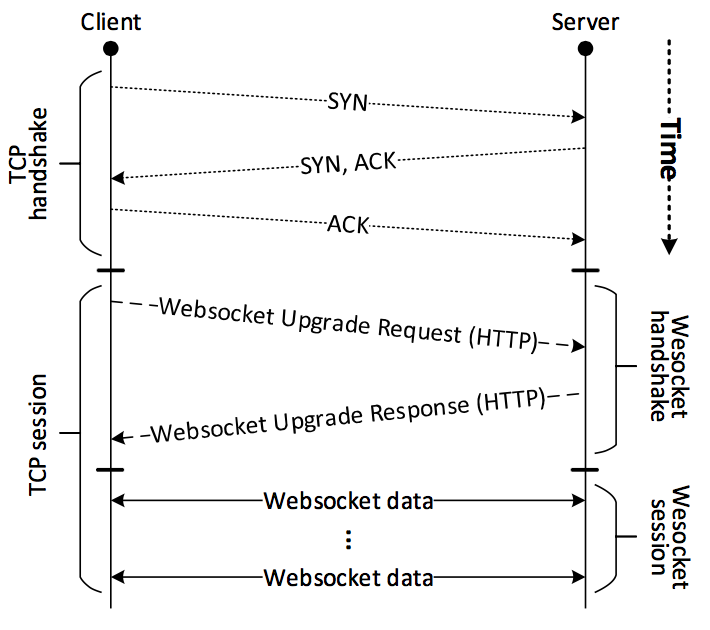
\includegraphics[width=\linewidth]{websocket_tcp_diagram.png}
    \caption{\ws-over-TCP sequence diagram (from \cite{performanceEvaluationOfWebsocketProtocol})}
    \label{fig:websocket_connection}
\end{figure}


\section{Performance of \ws{}}

As we saw in section~\ref{handshake}, establishing a \ws{} session requires at least five messages.
The cost of \ws{} connection establishment was evaluated to be 3.7 times longer than a TCP connection \cite{performanceEvaluationOfWebsocketProtocol}.  % evaluated to be

As observed in section~\ref{XHR}, XHR and XHR long polling were the two most common methods to simulate a full-duplex connection.
To determine whether \ws{} outperforms these, we are going to inspect the latency and the throughput of each of these techniques.
Moreover, we are going to see how good \ws{} performs compared to TCP. %the two most common methods to ... (pas besoin de used), how good \ws does/performs pas besoin de -ing :p

\subsection{Comparing the latency}

\begin{figure*}[!t]
    \centering
    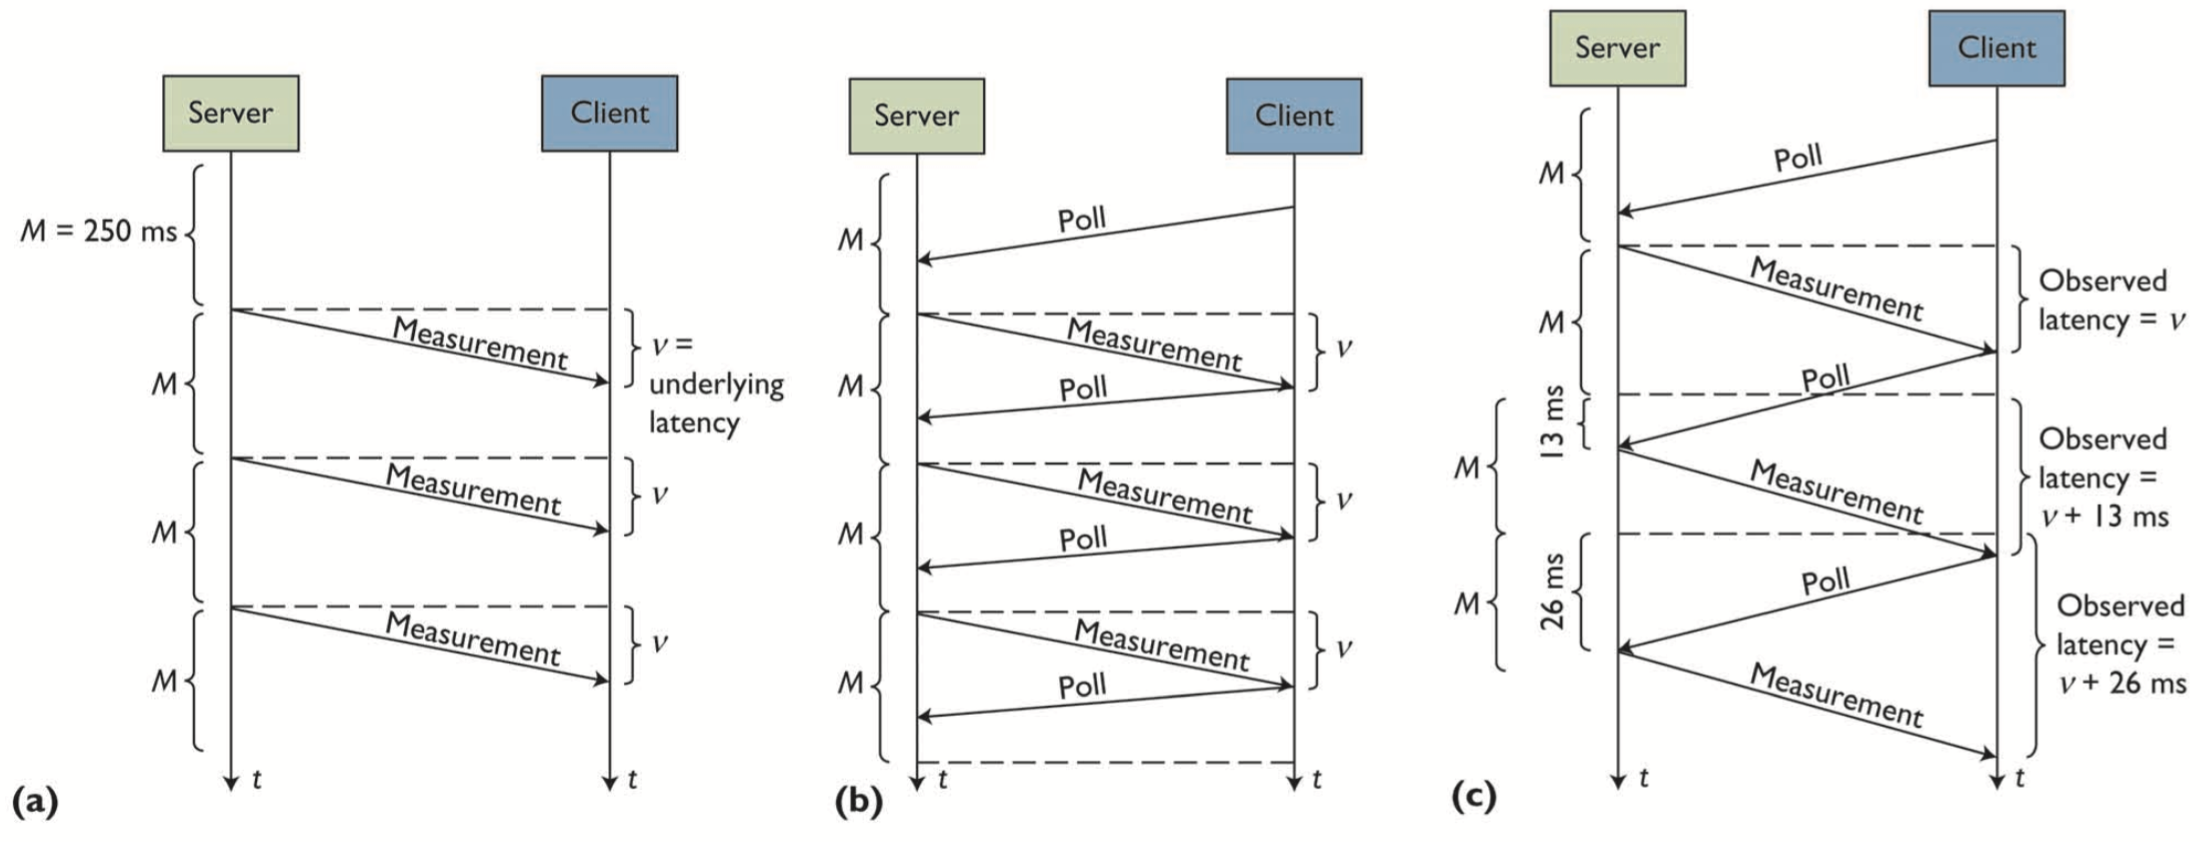
\includegraphics[width=\textwidth]{comdisp.png}
    \caption{Communication behavior in three situations. (a) is using \ws{}; (b) is using long polling with a low underlying latency; (c) is using long polling with a latency greater than half the data measurement rate. Measurements occur at a constant rate of one every $M$ ms. (from \cite{communicationAndDIsplayingRealTimeDataWithWebSocket})}
    \label{fig:comdisp}
\end{figure*}

The experimentation compares \ws{}, XHR and XHR long polling with different latencies in the underlying link.

In \cite{communicationAndDIsplayingRealTimeDataWithWebSocket}, the researchers imagine an experiment to measure the latency induced by the use of \ws{} compared to XHR and XHR long polling.
The server receives weather information every 250 ms from a wind sensor and serves it via several ways (WS, XHR and XHR LP).
To compare the latency, clients and servers are synchronized.

In this experiment, the XHR without long polling always achieves higher latency.
This is understandable given the fact the client has to periodically poll the server for new data.
The comparison with XHR is not helpful and will not be considered.

Figure~\ref{fig:comdisp}, from \cite{communicationAndDIsplayingRealTimeDataWithWebSocket}, presents three interesting communication behaviors.
Figure~\ref{fig:comdisp}a illustrates the \ws{} protocol behavior once it has successfully established the socket connection. Each time the server receives a measurement from the sensor, the server can immediately send the measurement to the client.
Figure~\ref{fig:comdisp}b illustrates the XHR long polling behavior with an underlying latency low enough ($< 125 $ms, which corresponds to half the $250$ms observation rate) for the client to establish a poll request that the server will keep until it receives a new measurement from the sensor. % new measurementS, ou a new mea...
Figure~\ref{fig:comdisp}c illustrates the XHR long polling behavior with an underlying latency higher than $125$ms.
The client first polls the server, the request arrives at the server before or at the exact time a measurement is available.
When a measurement is available, the server sends the message immediately from the sensor to the client, which closes the connection.
Thus, when the server receives a new poll request from the client, at least one sensor is in the client's queue.
The observed latency is greater than the underlying link.
The long polling is a viable situation as long as the underlying latency is less than half the data measurement rate.
In  situations (a) and (b) of the figure~\ref{fig:comdisp}, the observed latency is the underlying latency, meaning that XHR long polling can perform as good as \ws{}.



Another experiment in \cite{collinalatency} is performed over a simulated satellite link.
The researchers set up a dummy network introducing such a latency that the round trip time is fixed at $600$ms.
Then the server or the client has to send 100 messages of 39 bytes. The results are similar.
For \ws{} the average latency is of about $600$ms, the latency of the dummy network. And for the XHR long polling, the average latency is about $1200$ms, twice the delay introduced.
This makes sense as every time the client (resp. server) has to send (resp. receive) a message in XHR long polling, a new connection has to be established before the data can be issued.
The standard deviation of these values is low.
This is explained by the fact that the whole experiment was conducted on a small network without congestion.

\begin{figure}[!ht]
    \centering
    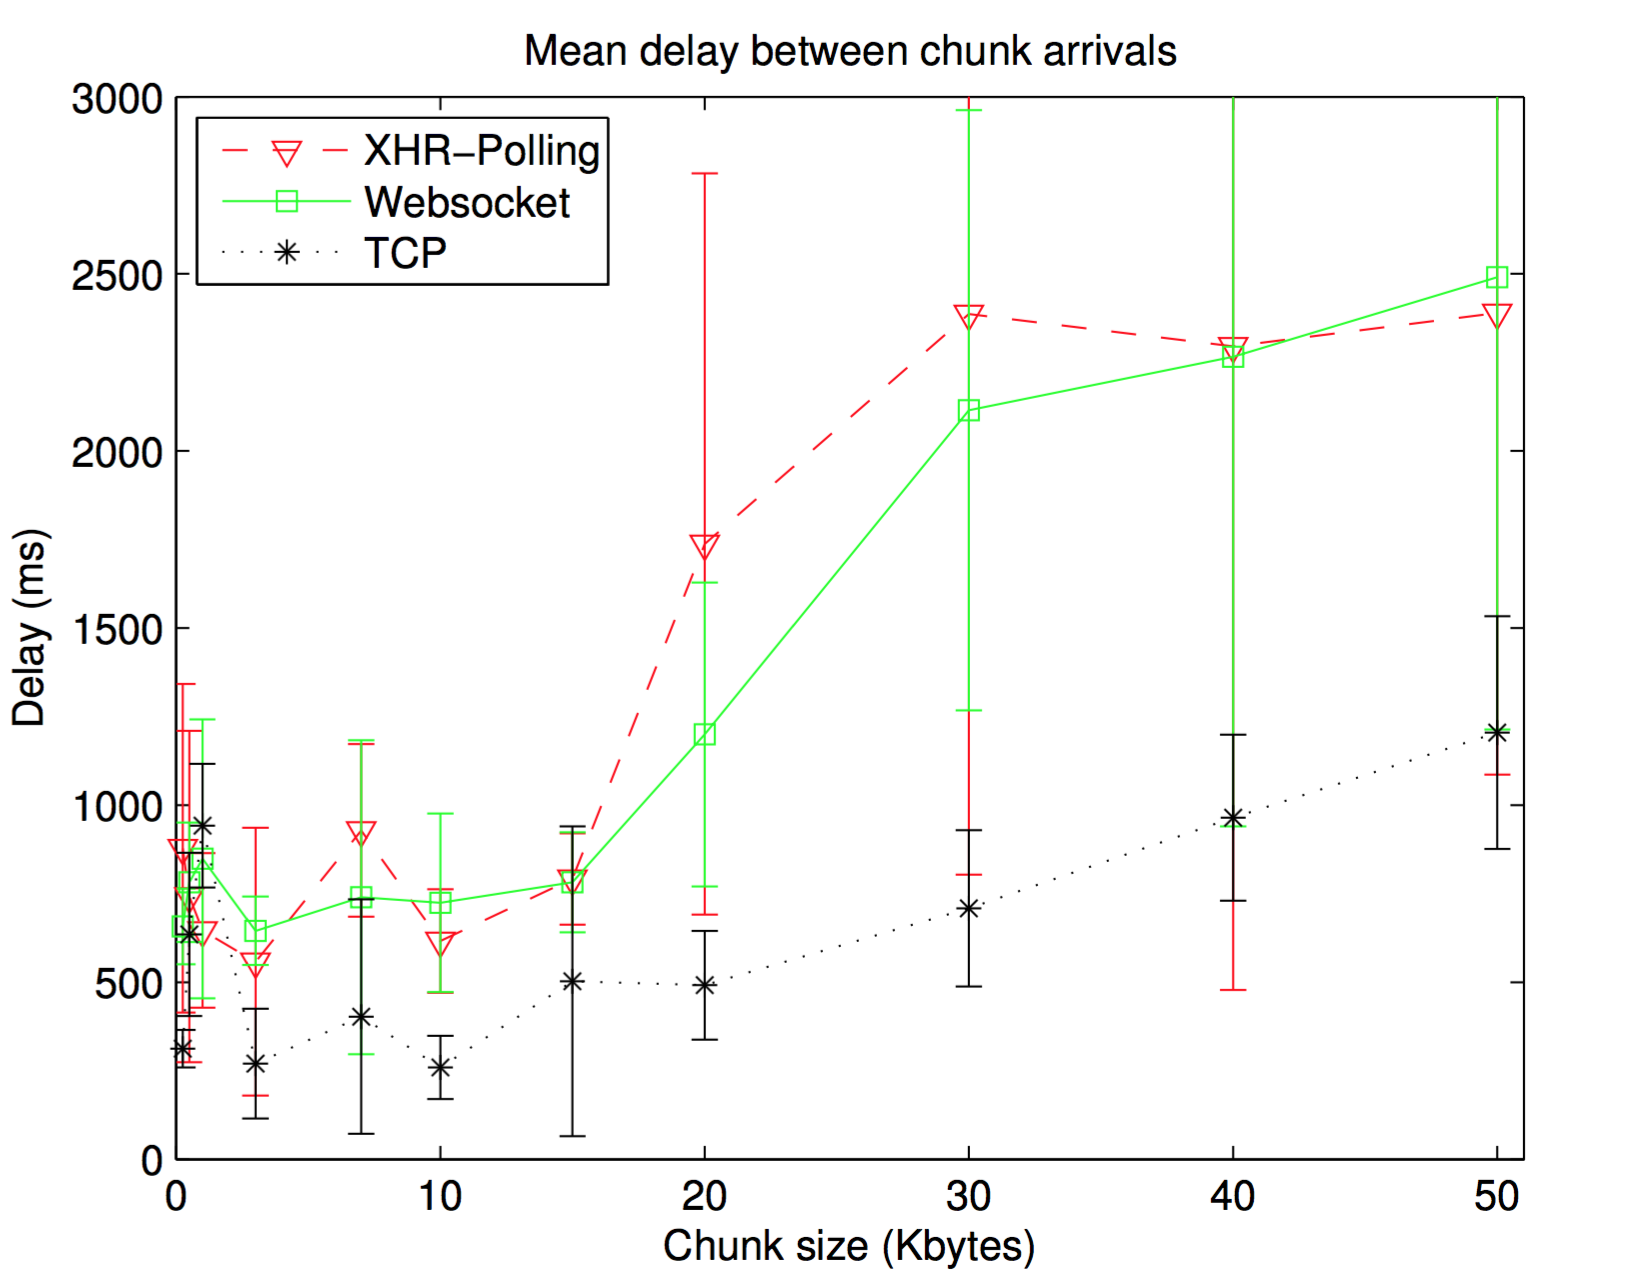
\includegraphics[width=\linewidth]{road.png}
    \caption{Delay over 3G cellular data network (from \cite{roadblock})}
    \label{fig:road}
\end{figure}

These experiments show that \ws{} achieves better performance than XHR.
But what about \ws{} versus plain TCP ?
This experiment was conducted in \cite{roadblock}.
The setup is a web application that is a simple data echo service.
Clients send a fixed-size chunk of random data to the server that simply sends it back to its respective client.
Figure~\ref{fig:road} shows the delays in receiving consecutive data chunks as a function of data chunk size. %the average delay (sans s) (y a bien qu'un delais qu'on mesure dont on fait la moyenne?)
This experiment is conducted on a 3G cellular data network with three different \mbox{protocols :} XHR long polling, \ws{} and TCP.
We are not going to rediscuss the results concerning \ws{} versus XHR long polling.
We can see that which other tests highlighted remains valid in this experiment. % "we can see that what" pas bon "that which" mais si moyen de reformuler mieux.
%The result of TCP versus \ws{} are questioning (QUESTIONABLE? QUESTIONED IN THIS PAPER?). -> questioned. 'fin j'imagine dépend de ce que tu veux dire.
The delay is increased by a factor of 2-3 when using \ws{} as compared to raw TCP. % The delay is increased by a factor of
Authors of this study conjectured that the reasons for these additional delays are due to additional buffering time, more chatty protocols, and additional overhead.
The first point is mentioned in the IETF HTML5 \ws{} specification ``the implementation MAY delay the actual transmission arbitrarily, e.g., buffering data so as to send fewer IP packets.'' \cite{rfc6455}.
Also, we can notice that the standard deviation is larger for \ws{} compared to TCP.
This standard deviation is called the jitter measurement in networking.
Authors of \cite{roadblock} made another experiment to measure the jitter of each of these protocols.
\begin{figure}[!ht]
    \centering
    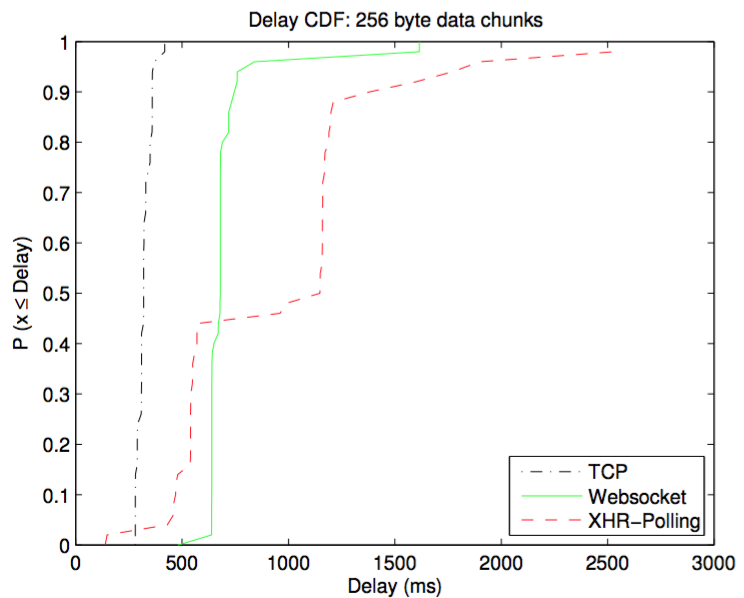
\includegraphics[width=\linewidth]{road_jitter.png}
    \caption{Cumulative distribution function of delays between 256-byte chunk arrivals (from \cite{roadblock})}
    \label{fig:road2}
\end{figure}

To do this, they measured the delay between successive 256-byte chunks. %to do this
The results are shown in figure~\ref{fig:road2}, in a cumulative distribution function.
The figure shows that, with TCP, we can expect that over 90\% of all data chunks will arrive at the client with an inter-chunk delay of 360ms or less. The corresponding numbers for \ws{} and XHR long polling are $760$ms and $1382$ms respectively. %over 90% au lieu de more than est plus lisible
There is a performance gap between TCP and \ws{} protocol.
This phenomenon is accentuated by the fact that the size of the chunks is small.
As the transmission delay is short for small chunks, the main factor of the latency depends on the underlying latency and the processing time of protocols.
To better understand the reason of this gap, we must analyze the generated overhead.

\subsection{Comparing overhead and throughput}

\begin{figure}[!ht]
    \centering
    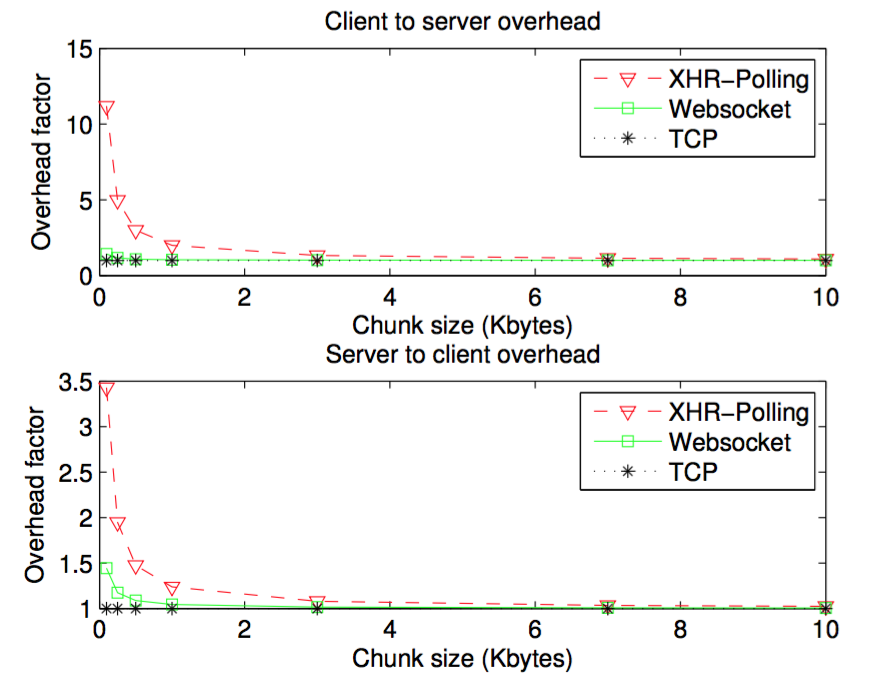
\includegraphics[width=\linewidth]{road4.png}
    \caption{Overhead over a traffic-shaped network (from \cite{roadblock})}
    \label{fig:road4}
\end{figure}

Authors of \cite{roadblock} also studied the throughput of the \ws{} compared to TCP and XHR long polling.
To do so, they used a new setup with a dummy network. % bieeenn, pas de "for doing this" pour une fois :D => :3
This dummy network will be used to create a traffic-shaped network which restricts total egress bandwidth to 512kbit/sec and introduces a fixed latency of 50ms.
It will also capture packets to compute the overhead.
The rest of the setup is the same as before, the size of the chunks is fixed and the web service is a simple echoing.
In figure~\ref{fig:road4}, they have measured the overhead induced by varying the chunks size. %pas faux, mais pas besoin du "s" au chunks
As we can see, the overhead for XHR long polling is very important.
For small chunks, it can be up to ten times the size of the data. % small chunk sizes
This is easy to understand as XHR uses HTTP.
Thus, the HTTP header is included in each request and response in XHR long polling.
And the HTTP header size is unpredictable as it contains a lot of superfluous information, such as browser cookies. % redundant au lieu de superfluous je dirais, information au singulier
It explains why the overhead from the client to the server is more important than the overhead from the server to the client as the client is more likely to add unnecessary headers.
We can see that the overhead factor for \ws{} is more reasonable.
This overhead is due to the header of the \ws{} protocol described in section~\ref{sec:ws-header}.
For a chunk of 256 bytes transmitted from the client to the server, the XHR long polling imposes a large overhead factor of up to 5 times the size of the chunk, Whereas the overhead factor of \ws{} is at 1.16. %5 times what ? 5 times the the chunk?
 % Whereas


\begin{figure}[!ht]
    \centering
    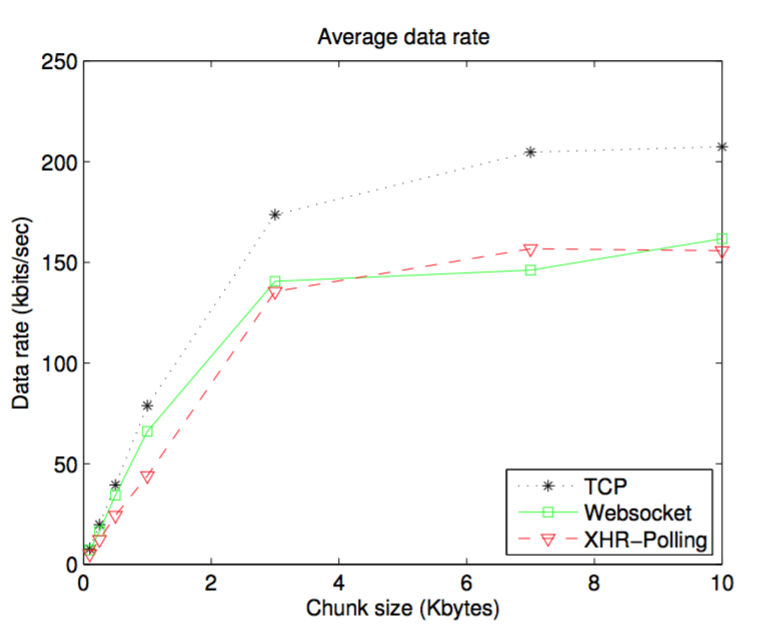
\includegraphics[width=\linewidth]{road3.png}
    \caption{Throughput (from \cite{roadblock})}
    \label{fig:road3}
\end{figure}

Authors of \cite{roadblock} also studied the throughput of the \ws{} compared to TCP and XHR long polling.
To do so, they used the same setup as described before (traffic-shaped network).
The figure~\ref{fig:road3} shows the net throughput (amount of useful data received, stripped of protocol overhead, in kbits/s) at the client as a function of data chunk sizes.
We can see that TCP performs better throughput than \ws{} and XHR long polling.
For a 1kB chunk, TCP achieves a throughput of 78kbits/s as compared to 66kbits and 44 kbits/s in the case of \ws{} and XHR long polling respectively.
We know that the throughput is dependent on the round trip time and the overhead, so these results are not surprising.

In \cite{EV}, authors also analyzed the performance of \ws{} throughput for electric vehicles communicating with \ws{}.
They have created an Android application simulating an electric vehicle.
The application uses the 3G cellular data network to communicate with a server.
They conclude that \ws{} is inefficient in comparison to regular TCP as TCP requires 40\%-50\% less bit rate than \ws{} for their messages.
The size of the status messages of their electric vehicles is of about 500 bytes.
As the message is shorter, the overhead ratio is higher.
These results are in agreement with the previous ones.
The authors highlight the fact that \ws{} may require keepalive traffic to keep the connection open due to the policy of some proxies. % can need? needs ou may need (et je mettrais require, pas need)
These keepalive messages can use a lot of unnecessary traffic, especially if the  amount of data exchanged is low. %These ... can use a lot of unnecessary traffic (ils dépensent rien, ils utilisent, c'est toi qui dépense :p)

%To reduce network utilization, they invented three methods in order to aggregate the %data.
%The first is time sampling, every T second, the EV sends informations.
%The second is distance sampling, every D meters, the EV sends informations.
%And the last one is the bundling.
%The data are sent in bundle.
%These three parameters are represented as a tuple (T,D,B).
%For instance, (0, 0, 1) means that there is no periodic and distance sampling and B=1 means that there is no bundling as the bundle contains only one sample.

\section{Security}

As mentioned in section~\ref{sec:ws}, \ws{} benefits from the HTTP's security model. Also, using existing HTTP infrastructures causes some problems. % as mentioned in ... benefits from THE security model ... thereby bizarre je trouve, je mettrais "its problems"

\subsection{Same origin security}

During the handshake, the browser adds the \ttt{Origin} header to the HTTP Upgrade request.
The server can accept or deny requests based on this header. %deny requests based
Also, if they do not share the same origin, it is possible to establish a connection thanks to the Cross Origin Request Sharing (CORS) \cite{talkingtoyourself}. %if they do not share the same origin,
The principle is the same as in HTTP.

\subsection{Proxies and black boxes}
\label{sec:key}
As the web is the most common way to communicate on the internet, there are a lot of proxies and black boxes that intercept the traffic going through port 80. %on the internet
These intermediaries might not understand what happens once the negotiation for \ws{} Upgrade is achieved and this can be problematic. % rajouter à la phase précédente?
When a proxy or black box does not understand what has happened, the traffic can be altered or discarded. % what has happened
This will make the \ws{} communication unusable.
This triggers a problem for the adoption of the \ws s.  %juste le progres, sonne étrange comme ça

But the most undesired behavior happens when a proxy caches the \ws{} frames.
As described in \cite{talkingtoyourself}, if a proxy is doing such a thing, an attacker can poison the cache of the proxy with malicious payload. %the proxy's cache, mais c'est bien comme ça
When a legitimate user behind the proxy wants to retrieve the \ws{}, he will get the malicious payload from the poisoned proxy's cache.
To counter this, a masking key is sent by the client within the header of \ws{}, this key will be used by the server to mask the payload by applying a xor operation between the masking key and the payload.
As the client knows the masking key, it can decode the payload and be sure that the payload was not modified by any proxies or black boxes.
This mechanism defeats the cache poisoning attack.

\subsection{TLS}
\ws{} supports TLS.
This is useful to cipher payload but not only as proxies and black boxes can do nothing with TLS communication, by ensuring that a website is using secure \ws{}, it also ensures that no proxy or black box will prevent the connection.


\section{Conclusion}
In this paper, we covered the different solutions that were used prior to the \ws{}.
These include XHR polling and XHR long-polling.
Then, we introduced the \ws{}, which is composed of the \ws{} JavaScript API and the underlying \ws{} protocol. %composed of pas by
We saw that the \ws{} protocol was based on TCP.
We presented how two hosts could connect to each other to create a \ws{} session.
We also exposed the \ws{} header to explain the \ws{} frame structure. %exposed un peu bizarre mais bon
We ended the paper by comparing the technology with the prior solutions, with a focus on the throughput and the latency.
It turns out that the \ws{} causes lower performance compared to the plain TCP protocol.
It causes some overhead and has a higher latency than a plain TCP connection.
However, it is still better than the alternative solutions, like XHR polling and XHR long-polling. %like pas as XHR...
The overhead caused by the \ws{} is negligible for practical use, and for situations where a lot of data is sent, the initial HTTP handshake is amortized by the large number of payload transfers. %a lot of data is sent, the initial HTTP handshake is ...

% Rajouter une conclusion sur les quelques points de sécurité abordés
From a security point of view, we saw the threats that exist and how \ws{} counters these.
We also explained the importance of the masking key in the \ws{} frames sent by the clients. %capital à Masking ici?

Finally, we can conclude this paper by stating that the \ws{} protocol is a useful addition to the Web, which brings a full-duplex communication that is more efficient than the other solutions which try to simulate an equivalent behavior in HTTP-based applications.

\ifCLASSOPTIONcaptionsoff
  \newpage
\fi


\bibliographystyle{IEEEtran}
\bibliography{bibi}


\end{document}
